%%%%%%%%%%%%%%%%%%%%%%%%%%%%%%%%%%%%%%%%%
% Beamer Presentation
% LaTeX Template
% Version 1.0 (01/07/19)
%
%%%%%%%%%%%%%%%%%%%%%%%%%%%%%%%%%%%%%%%%%

%----------------------------------------------------------------
%	PACKAGES AND THEMES		-----------------------------------
%----------------------------------------------------------------

\documentclass[xcolor=table,11pt]{beamer}

\mode<presentation> {
	
	\usetheme{Frankfurt}
	\usecolortheme{dove}
	\usefonttheme{serif}
	
}
\usepackage{newtxtext,newtxmath}
\usepackage{graphicx}
\usepackage{booktabs} 
\usepackage{subfig}
\usepackage{pgf}
\usepackage{multirow}
\usepackage{appendixnumberbeamer}
\usepackage{bookmark}
\usepackage{siunitx}
\usepackage{animate}
\usepackage{xcolor}
\usepackage{soul}
\usepackage{pifont}
\usepackage{caption}
\usepackage{array}
\usepackage{pgffor}
\captionsetup{skip=0pt,belowskip=0pt}


%----------------------------------------------------------------
%	GENERAL OPTIONS 	-----------------------------------------
%----------------------------------------------------------------

% Set template options
\setbeamertemplate{section in toc}{\inserttocsectionnumber.~\inserttocsection}
\setbeamertemplate{frametitle}{\vspace*{1em}\insertframetitle}
\setbeamertemplate{enumerate items}[default]
\setbeamercolor{section in head/foot}{fg=white, bg=black}

% Headline
\makeatletter
\setbeamertemplate{headline}
{%
	\pgfuseshading{beamer@barshade}%
	\vskip-5ex%
	\begin{beamercolorbox}[ignorebg,ht=2.25ex,dp=3.75ex]{section in head/foot}
		\insertsectionnavigationhorizontal{\paperwidth}{\hskip0pt plus1fill}{\hskip0pt plus1fill}
	\end{beamercolorbox}%
	\ifbeamer@sb@subsection%
	\begin{beamercolorbox}[ignorebg,ht=2.125ex,dp=1.125ex,%
		leftskip=.3cm,rightskip=.3cm plus1fil]{subsection in head/foot}
		\usebeamerfont{subsection in head/foot}\insertsubsectionhead
	\end{beamercolorbox}%
	\fi%
}%
\makeatother

% Footline
\makeatletter
\setbeamertemplate{footline}
{
	\leavevmode%
	\hbox{%
		\begin{beamercolorbox}[wd=.333333\paperwidth,ht=2.25ex,dp=1ex,left]{section in head/foot}%
			\usebeamerfont{author in head/foot}\hspace{10pt}\insertshortauthor
		\end{beamercolorbox}%
		\begin{beamercolorbox}[wd=.333333\paperwidth,ht=2.25ex,dp=1ex,center]{section in head/foot}%
			\usebeamerfont{title in head/foot}\insertshorttitle
		\end{beamercolorbox}%
		\begin{beamercolorbox}[wd=.333333\paperwidth,ht=2.25ex,dp=1ex,right]{section in head/foot}%
			\usebeamerfont{date in head/foot}\insertshortdate{}\hspace*{2em}
			\insertframenumber{}\hspace*{2em}
	\end{beamercolorbox}}%
	\vskip0pt%
}
\makeatother

% Add logo
\logo{\pgfputat{\pgfxy(0,7)}{\pgfbox[right,base]{
\includegraphics[width=0.1\paperwidth]{Unibe_Logo}}}}
% \titlegraphic{\includegraphics[width=0.5\paperwidth]{Pictures/ESB_2023}}

% Table settings
\renewcommand{\arraystretch}{2}
\captionsetup{labelformat=empty,labelsep=none}
\definecolor{Gray}{gray}{0.9}

% Define highlitghing command
\makeatletter
\let\HL\hl
\renewcommand\hl{%
	\let\set@color\beamerorig@set@color
	\let\reset@color\beamerorig@reset@color
	\HL}
\makeatother

% Add overview at each begin of section
%\AtBeginSection[]
%{
	%	\begin{frame}
		%		\frametitle{Overview}
		%		\tableofcontents[currentsection]
		%	\end{frame}
	%}


\renewcommand{\arraystretch}{1.4}
\newcommand{\ColWidth}{1}
\newcommand{\TrimSize}{50}

%----------------------------------------------------------------
%	TITLE PAGE 	-------------------------------------------------
%----------------------------------------------------------------

\title[FABCORT]{Fabric-Elasticity Relationships in Cortical Bone} 

\author[mathieu.simon@unibe.ch]{\tiny{\bf{Mathieu Simon}}}

\medskip
\date{\today}

\begin{document}
	
	\begin{frame}
		\titlepage
	\end{frame}
	
	%----------------------------------------------------------------
	%----------------------------------------------------------------
	%----------------------------------------------------------------
	
	\section{Material and Methods}

	\begin{frame}
		\frametitle{Samples}
		\begin{columns}
			\column{0.5\linewidth}

			Bone matrix
			\begin{itemize}
				\item Franzoso et al. \cite{p1}
				\item Dall'Ara et al. \cite{p2}
			\end{itemize}

			Cortical bone
			\begin{itemize}
				\item Femur
				\item \textmu CT at 6.5 \textmu m voxel size
				\item RUS measurement
			\end{itemize}

			Trabecular bone
			\begin{itemize}
				\item Tibia
				\item HR-pQCT at 61 \textmu m voxel size
			\end{itemize}

			\column{0.5\linewidth}
			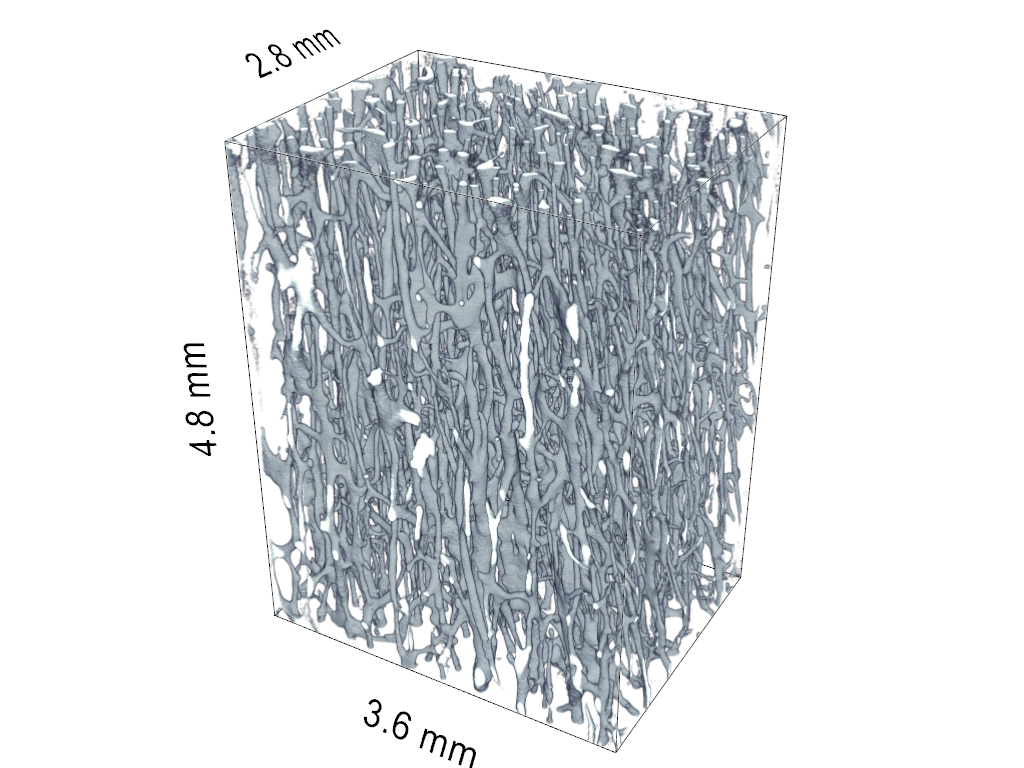
\includegraphics[width=\linewidth]{../Results/Scans/2009_213_L}
		\end{columns}
	\end{frame}

	\begin{frame}
		\frametitle{Numerical Analysis}
		\begin{columns}
			\column{0.45\linewidth}
			Cortical bone
			\begin{itemize}
				\item 16x 1mm\textsuperscript{3} ROIs
				\item Fabric (Medtool)
				\item Coarsening factor 2
				\item Homogenisation (Abaqus)\\
					  Transverse isotropic\\
					  Isotropic
			\end{itemize}
			\vfill
			Trabecular bone
			\begin{itemize}
				\item Homogenisation (Abaqus)\\
					  Isotropic
			\end{itemize}

			\column{0.5\linewidth}
			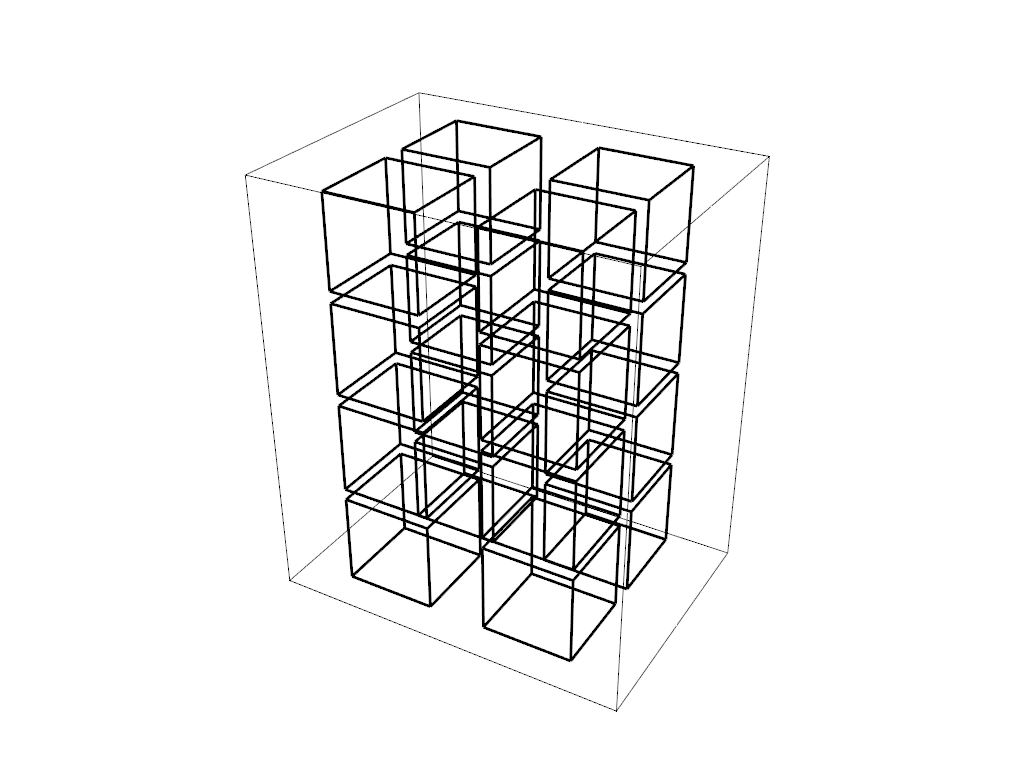
\includegraphics[width=\linewidth]{../Results/ROIs/ROIs}
		\end{columns}
	\end{frame}

	\begin{frame}
		\frametitle{Comparison to Experiment}
		\framesubtitle{Cortical ROIs}
		Analysis pipeline
		\begin{itemize}
			\item Homogenisation with tranverse isotropic matrice
			\item Average 16 tensors
			\item ROI's CV < 0.263
			\item Project to transverse isotropy
			\item Linear regression (BV/TV and $\mathbb{S}$)
			\item $\mathbb{S}$ and $\mathbb{E}$ anisotropy
		\end{itemize}
	\end{frame}

	\begin{frame}
		\frametitle{Cortical and Trabecular}
		\vfill Cortical and Trabecular Fabric\\
		\vfill Cortical and Trabecular CV vs BV/TV\\
		\vfill Cortical Constitutive Models
		\begin{itemize}
			\item Zysset-Curnier in orthotropic space
			\item Zysset-Curnier in transverse isotropic space
			\item Yang and Cowin in transverse isotropic space
		\end{itemize}
		\vfill Cortical and trabecular
		\begin{itemize}
			\item Transverse isotropic space
			\item Yang and Cowin model
		\end{itemize}
	\end{frame}

	%----------------------------------------------------------------
	%----------------------------------------------------------------
	%----------------------------------------------------------------
	
	\section{Results}

	\begin{frame}
		\frametitle{Comparison to Experiment}
		\framesubtitle{BV/TV and Stiffness}
		\centering
		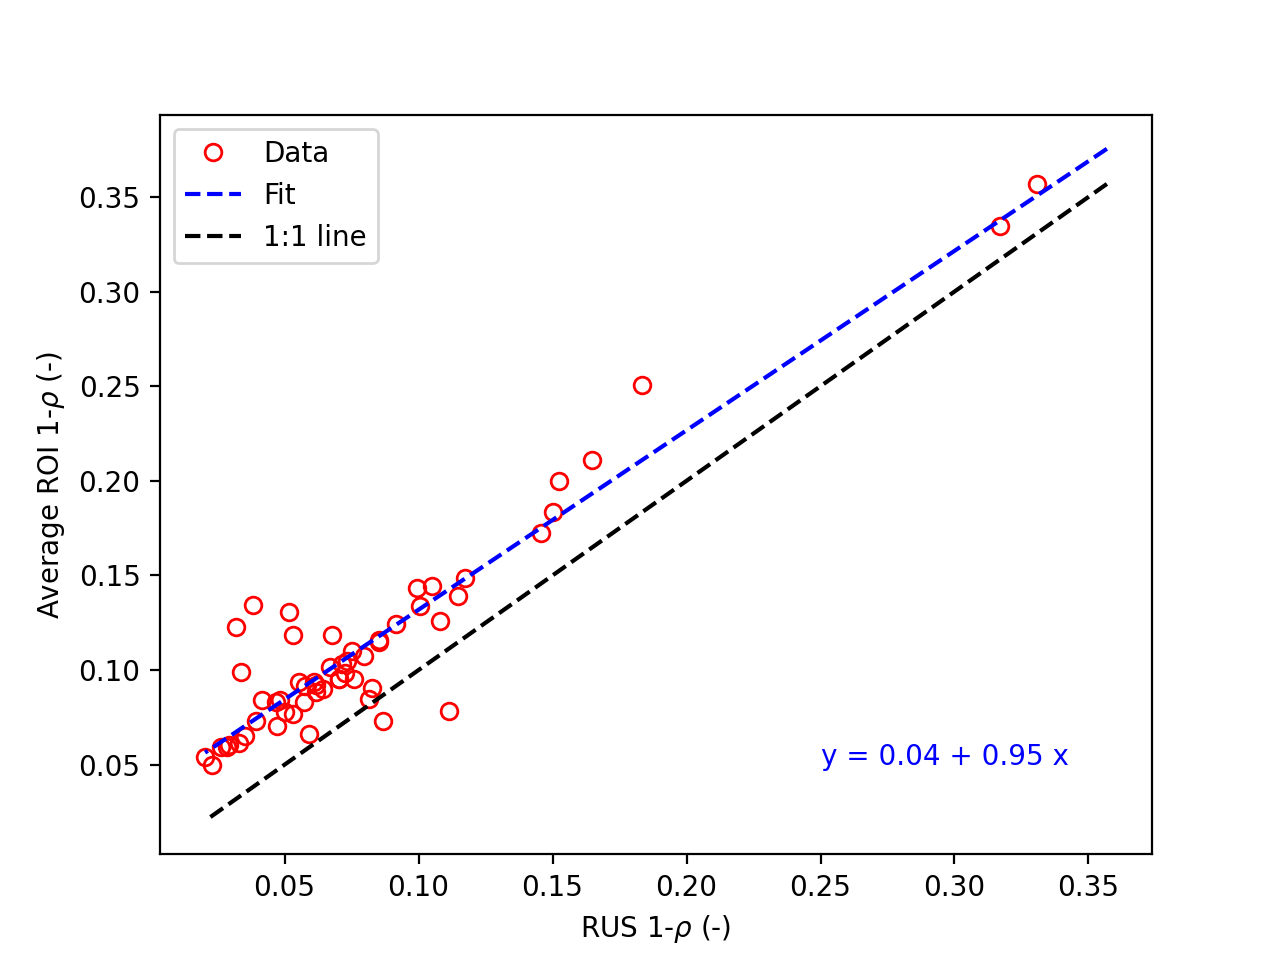
\includegraphics[height=0.35\linewidth]{../Results/ExpSim_Rho}
		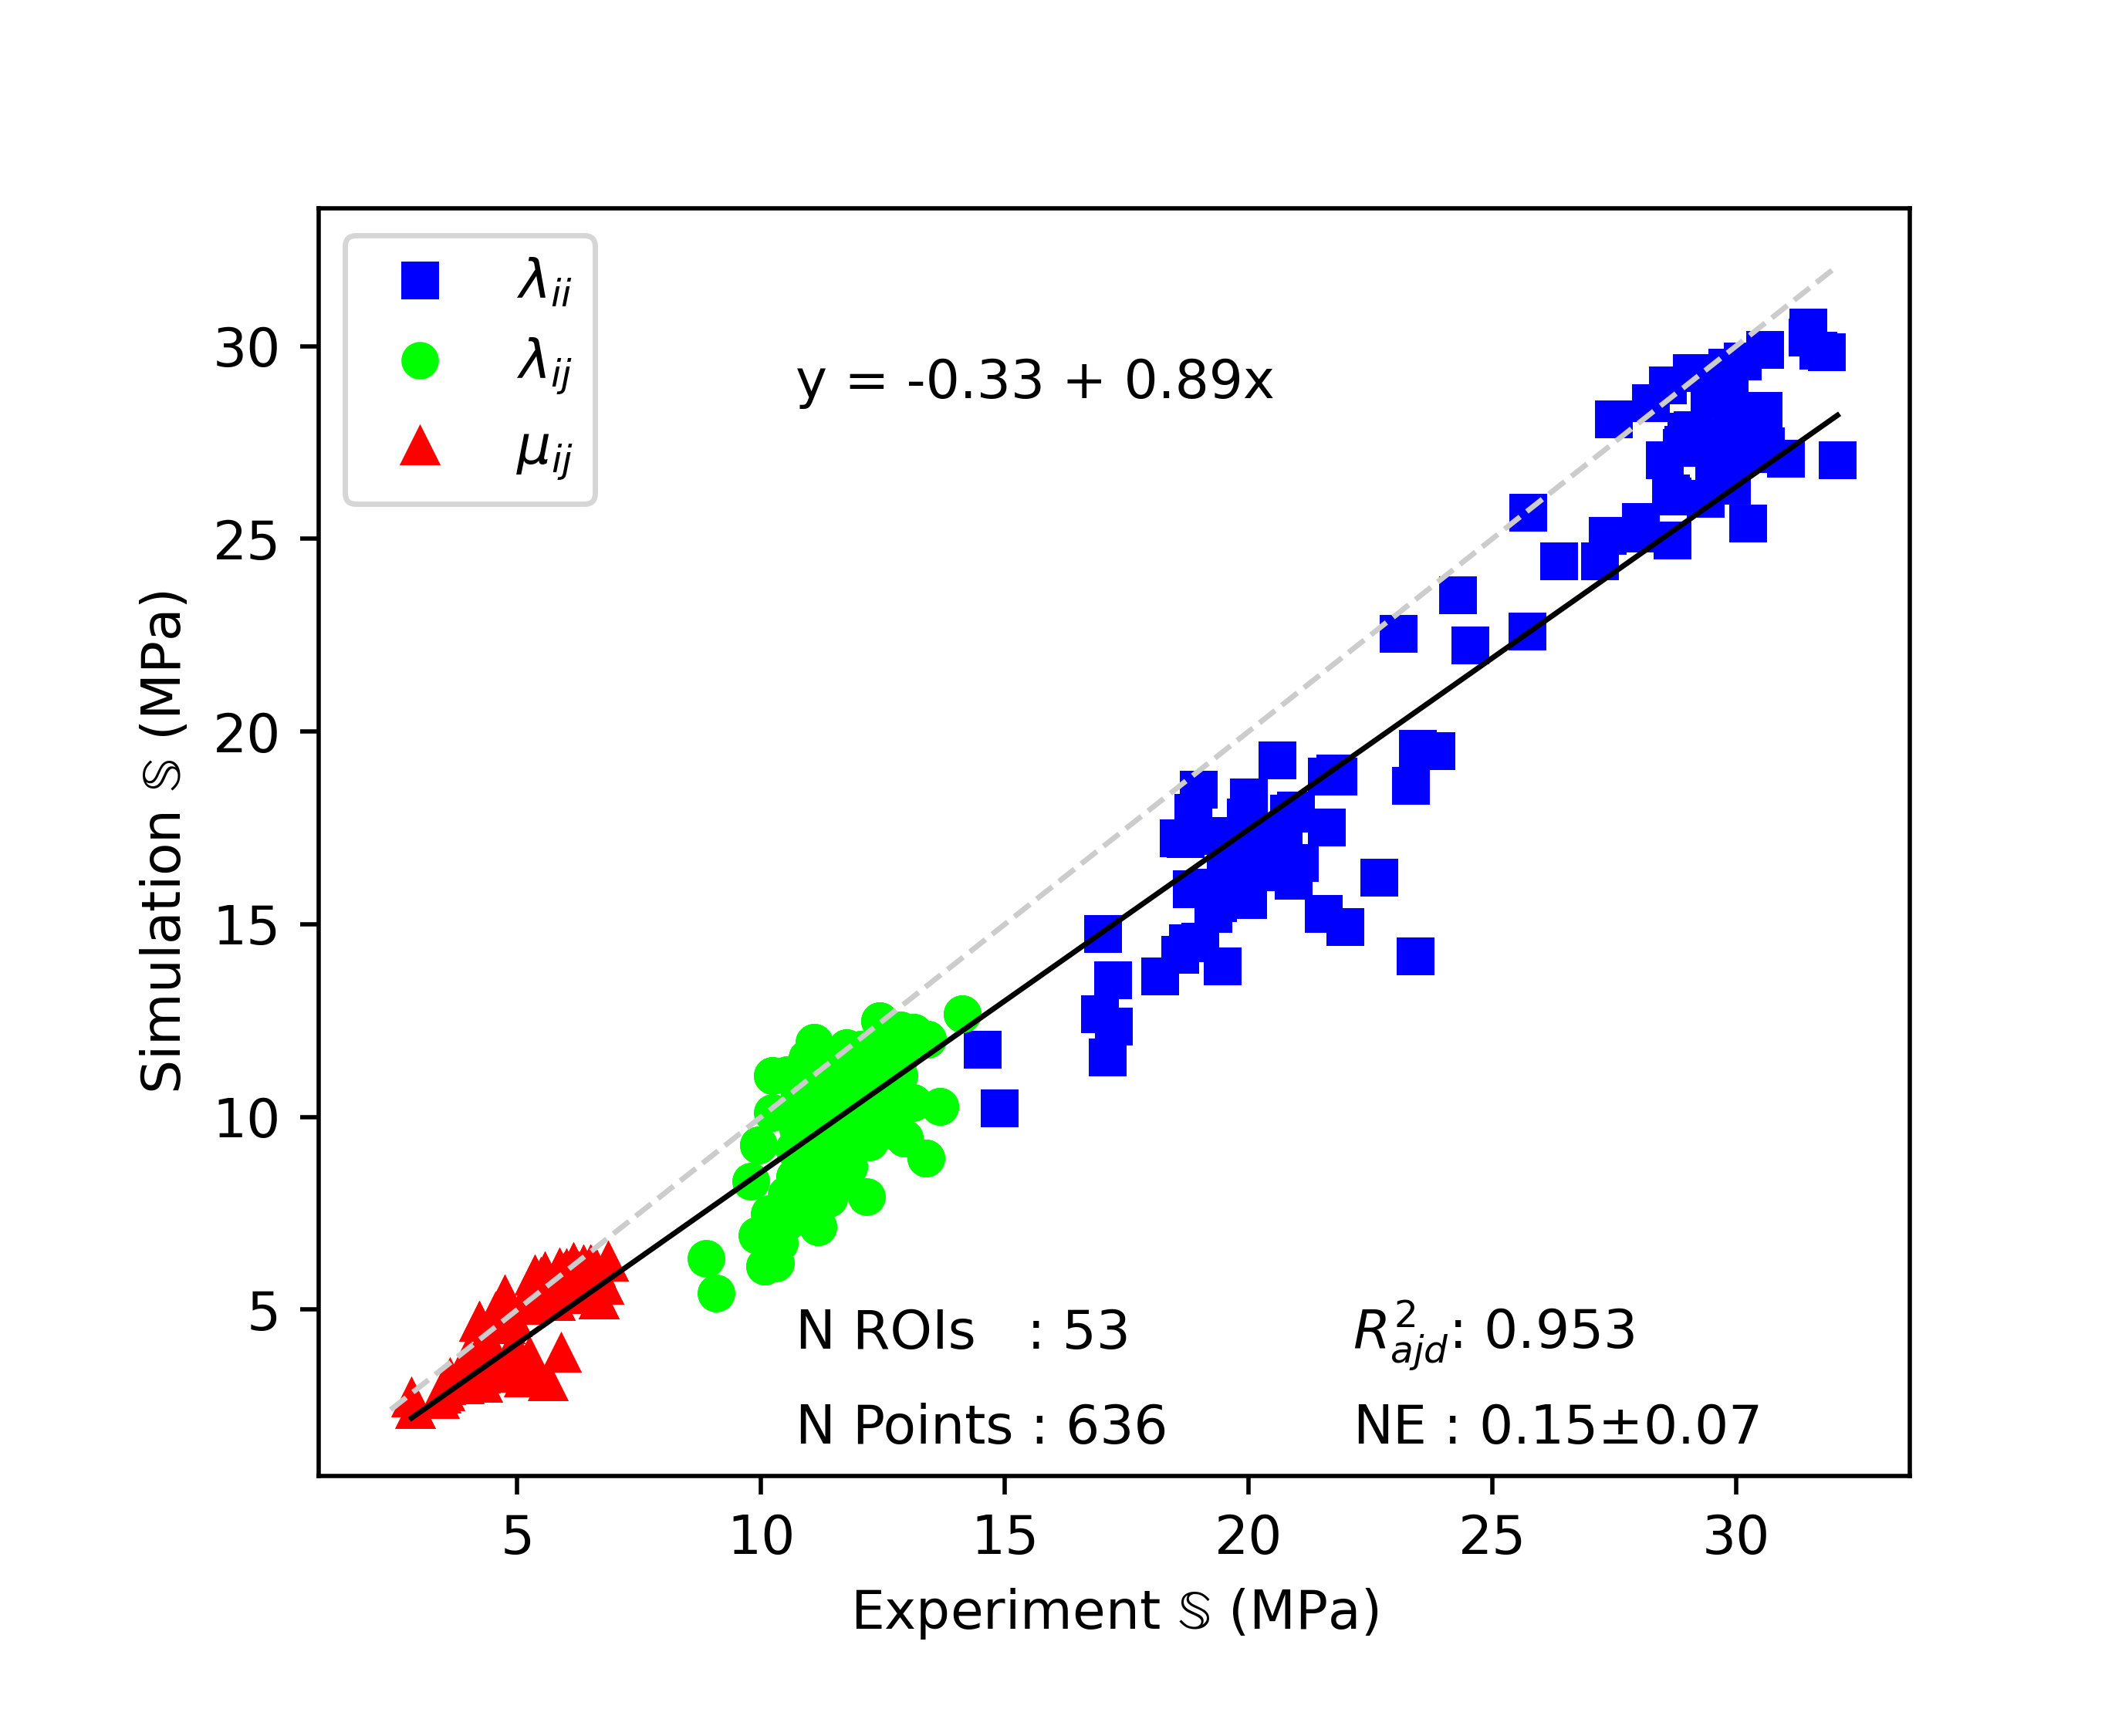
\includegraphics[height=0.35\linewidth]{../Results/ExpSim_S_Filt}
	\end{frame}

	\begin{frame}
		\frametitle{Comparison to Experiment}
		\framesubtitle{Stiffness and Compliance Anisotropy}
		\centering
		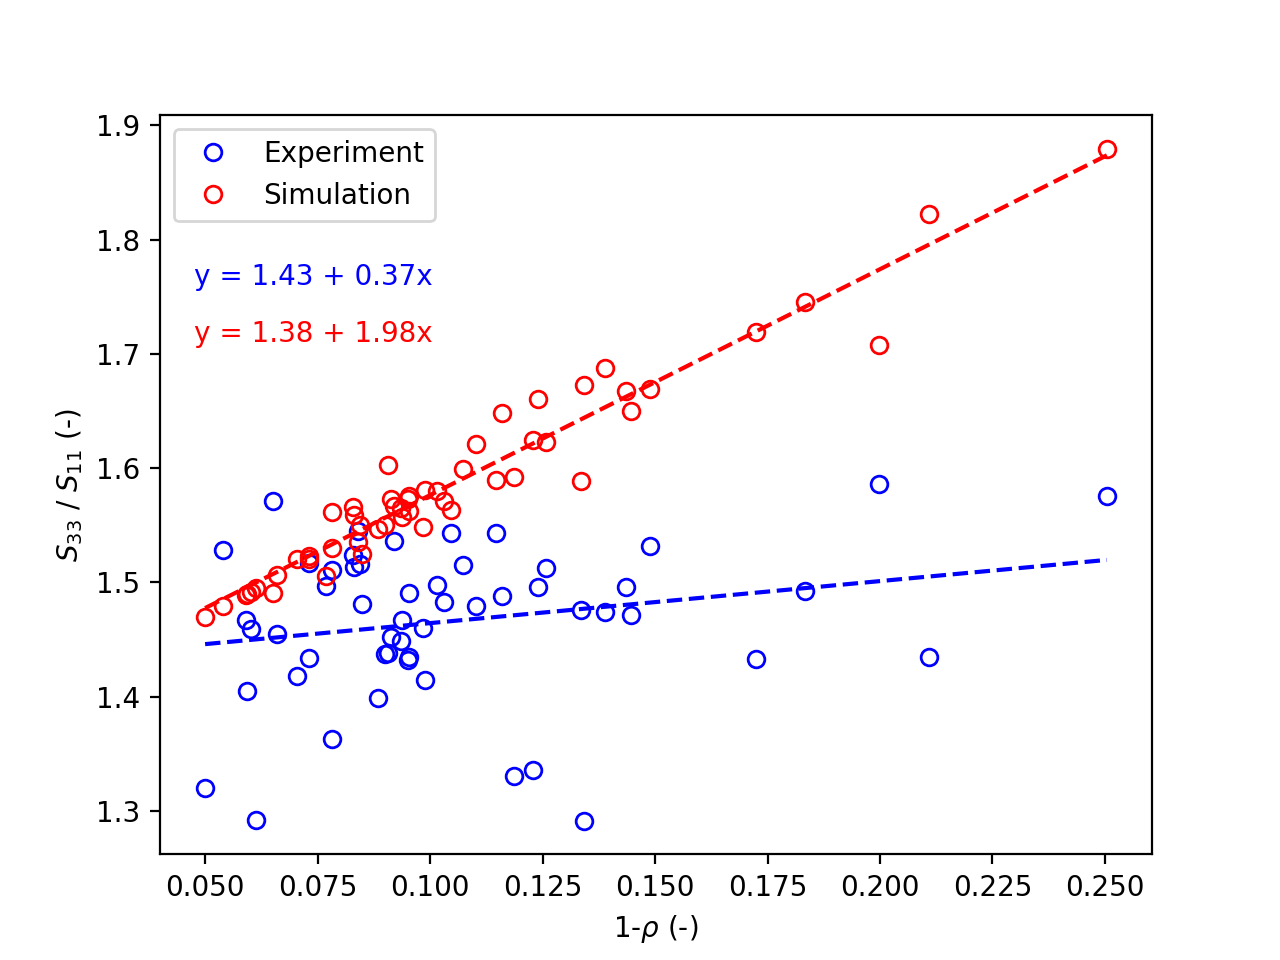
\includegraphics[height=0.35\linewidth]{../Results/ExpSim_AniS}
		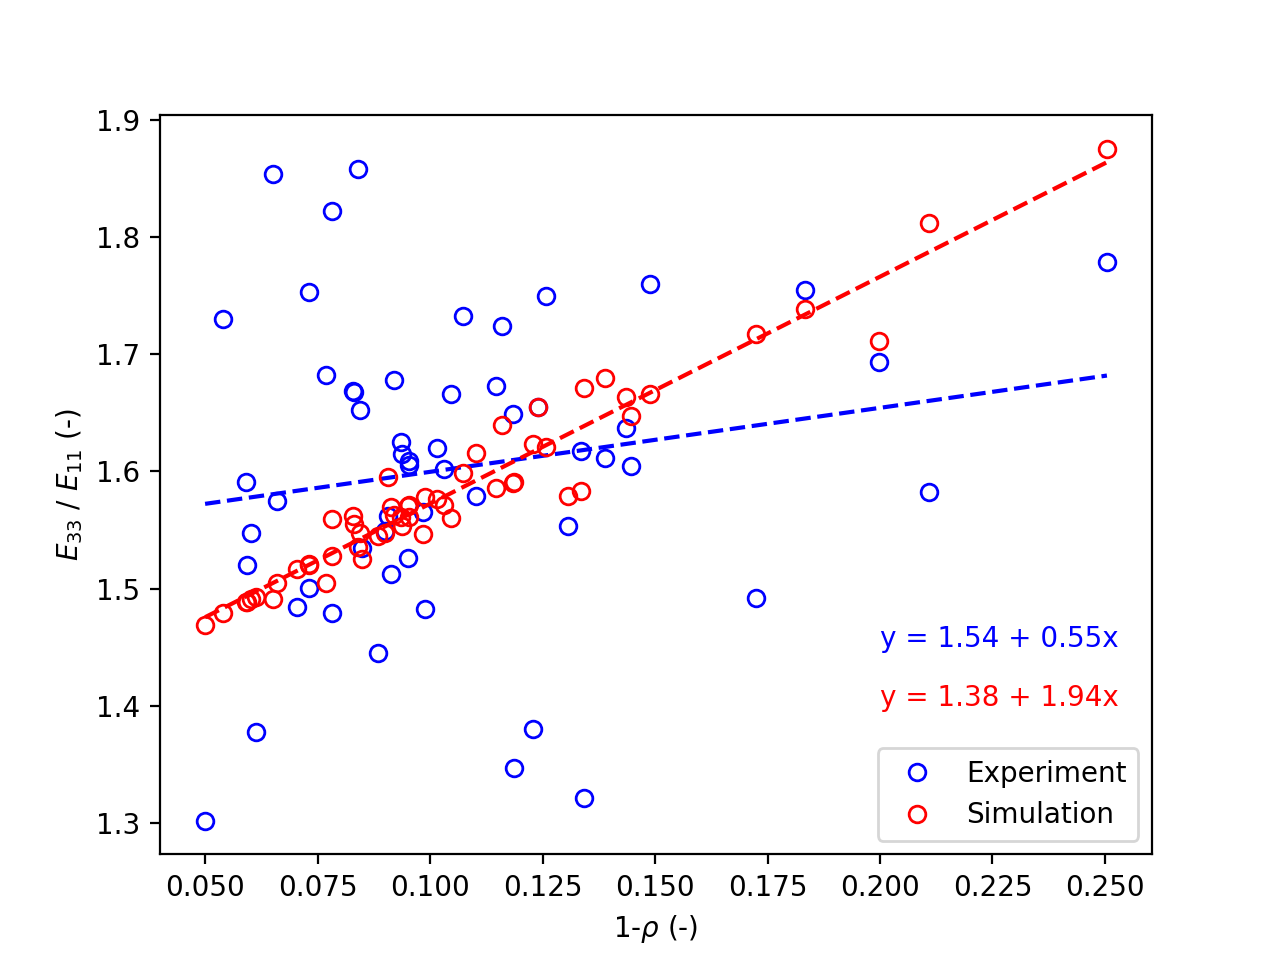
\includegraphics[height=0.35\linewidth]{../Results/ExpSim_AniE}
	\end{frame}

	\begin{frame}
		\frametitle{Cortical Bone}
		\framesubtitle{Fabric}
		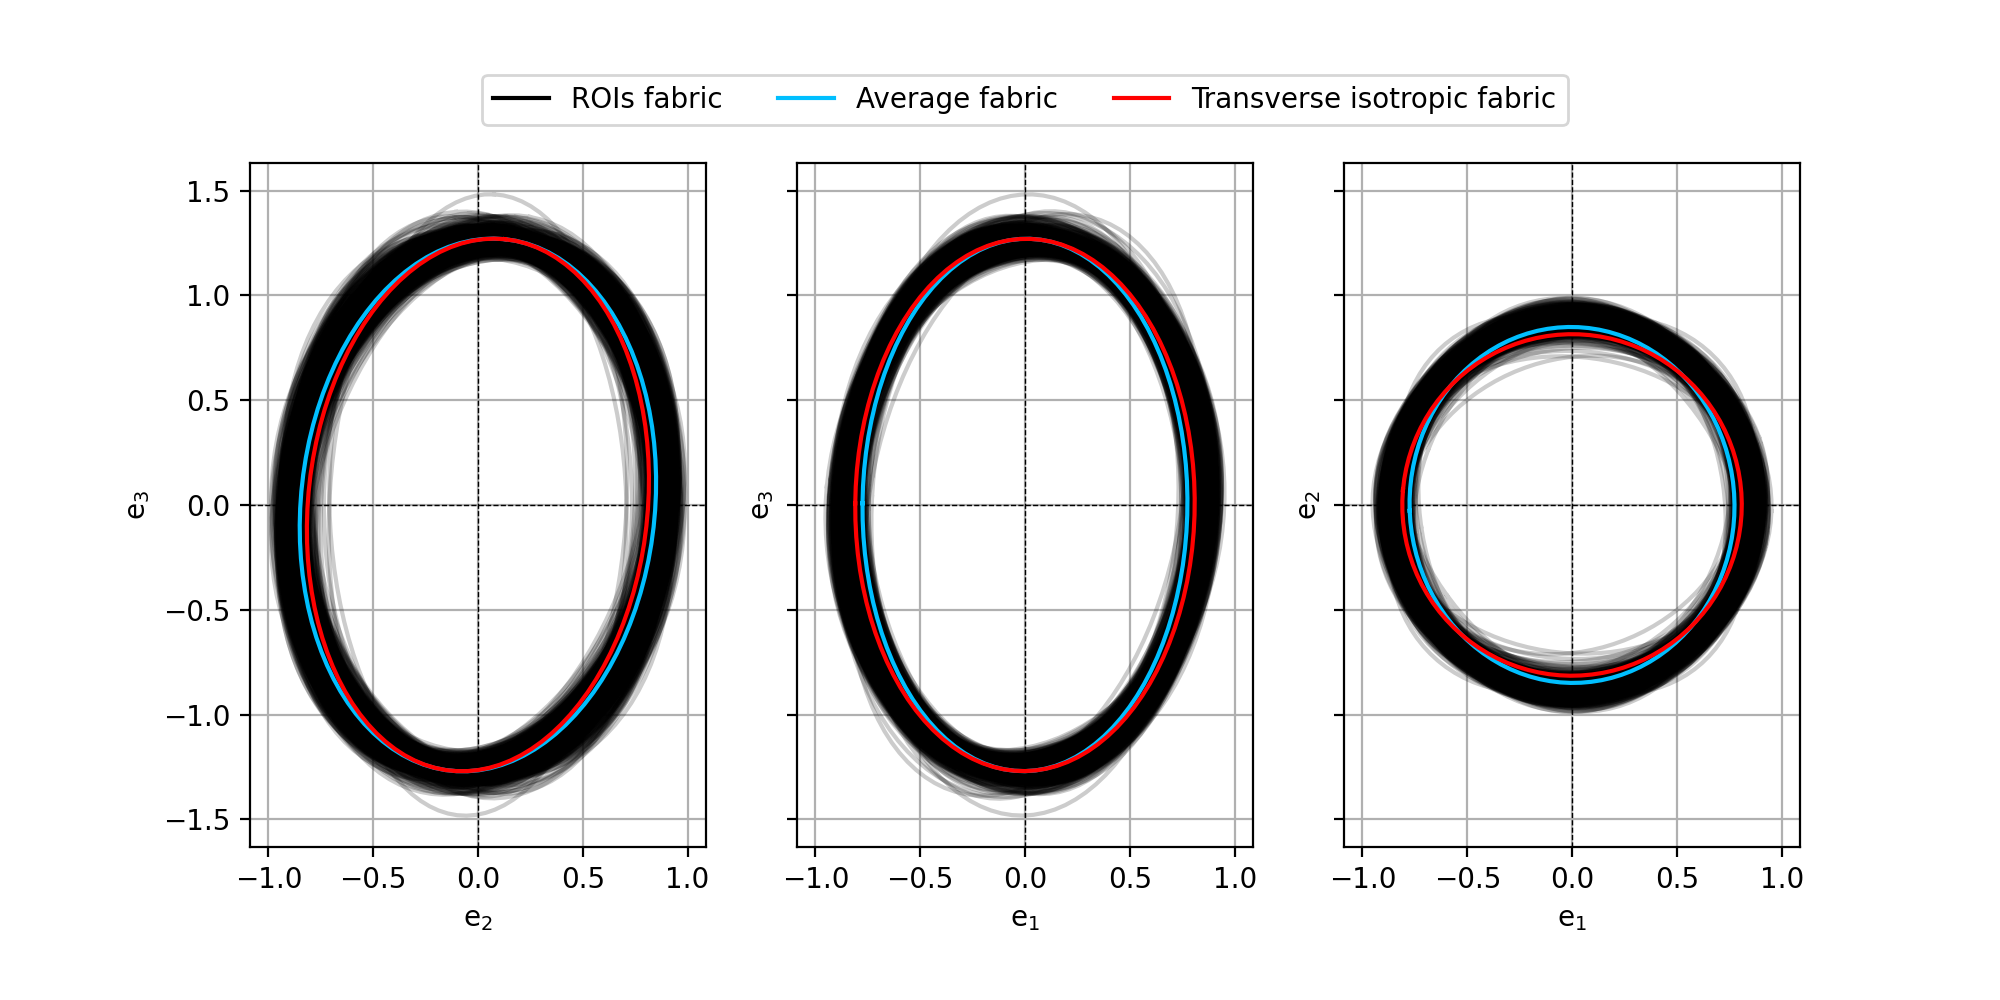
\includegraphics[width=\linewidth]{../Results/Fabric/Fabric}
	\end{frame}

	\begin{frame}
		\frametitle{Cortical and Trabecular Bone}
		\framesubtitle{BV/TV and CV}
		\centering
		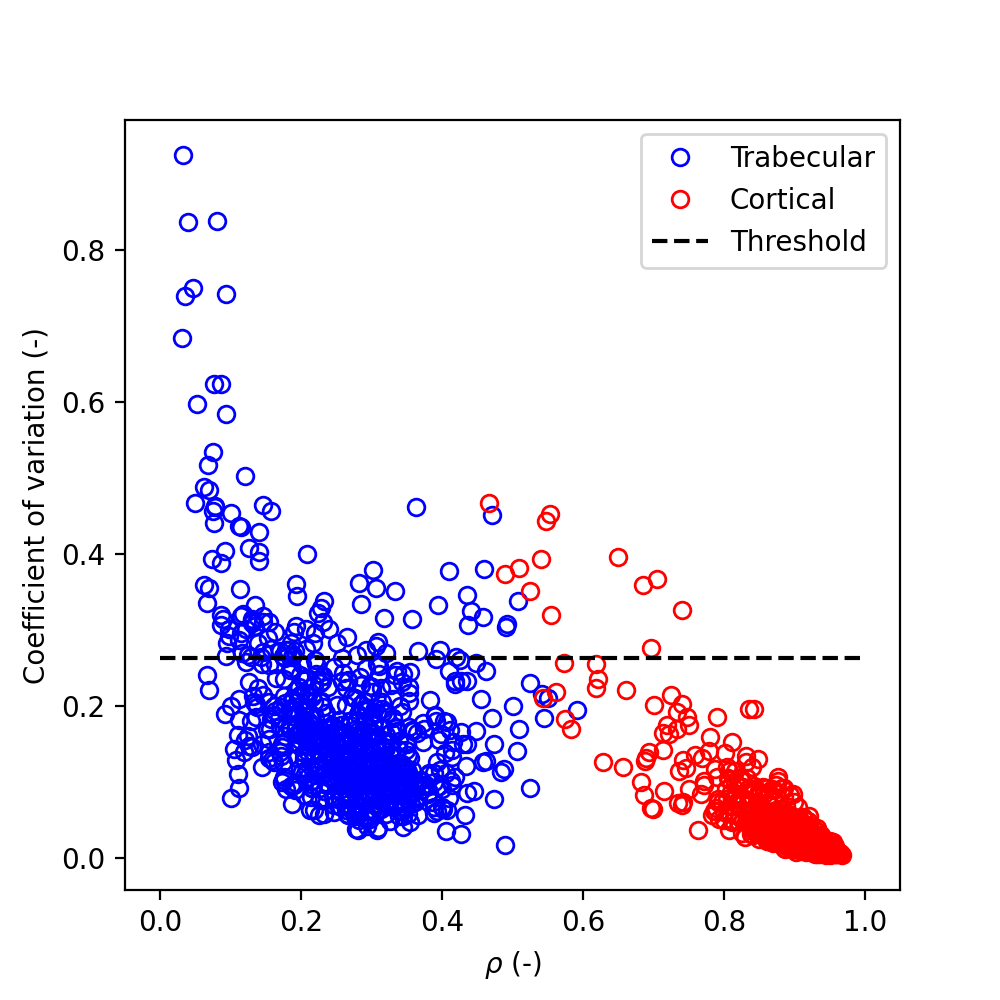
\includegraphics[height=0.425\linewidth]{../Results/CV_Rho}
		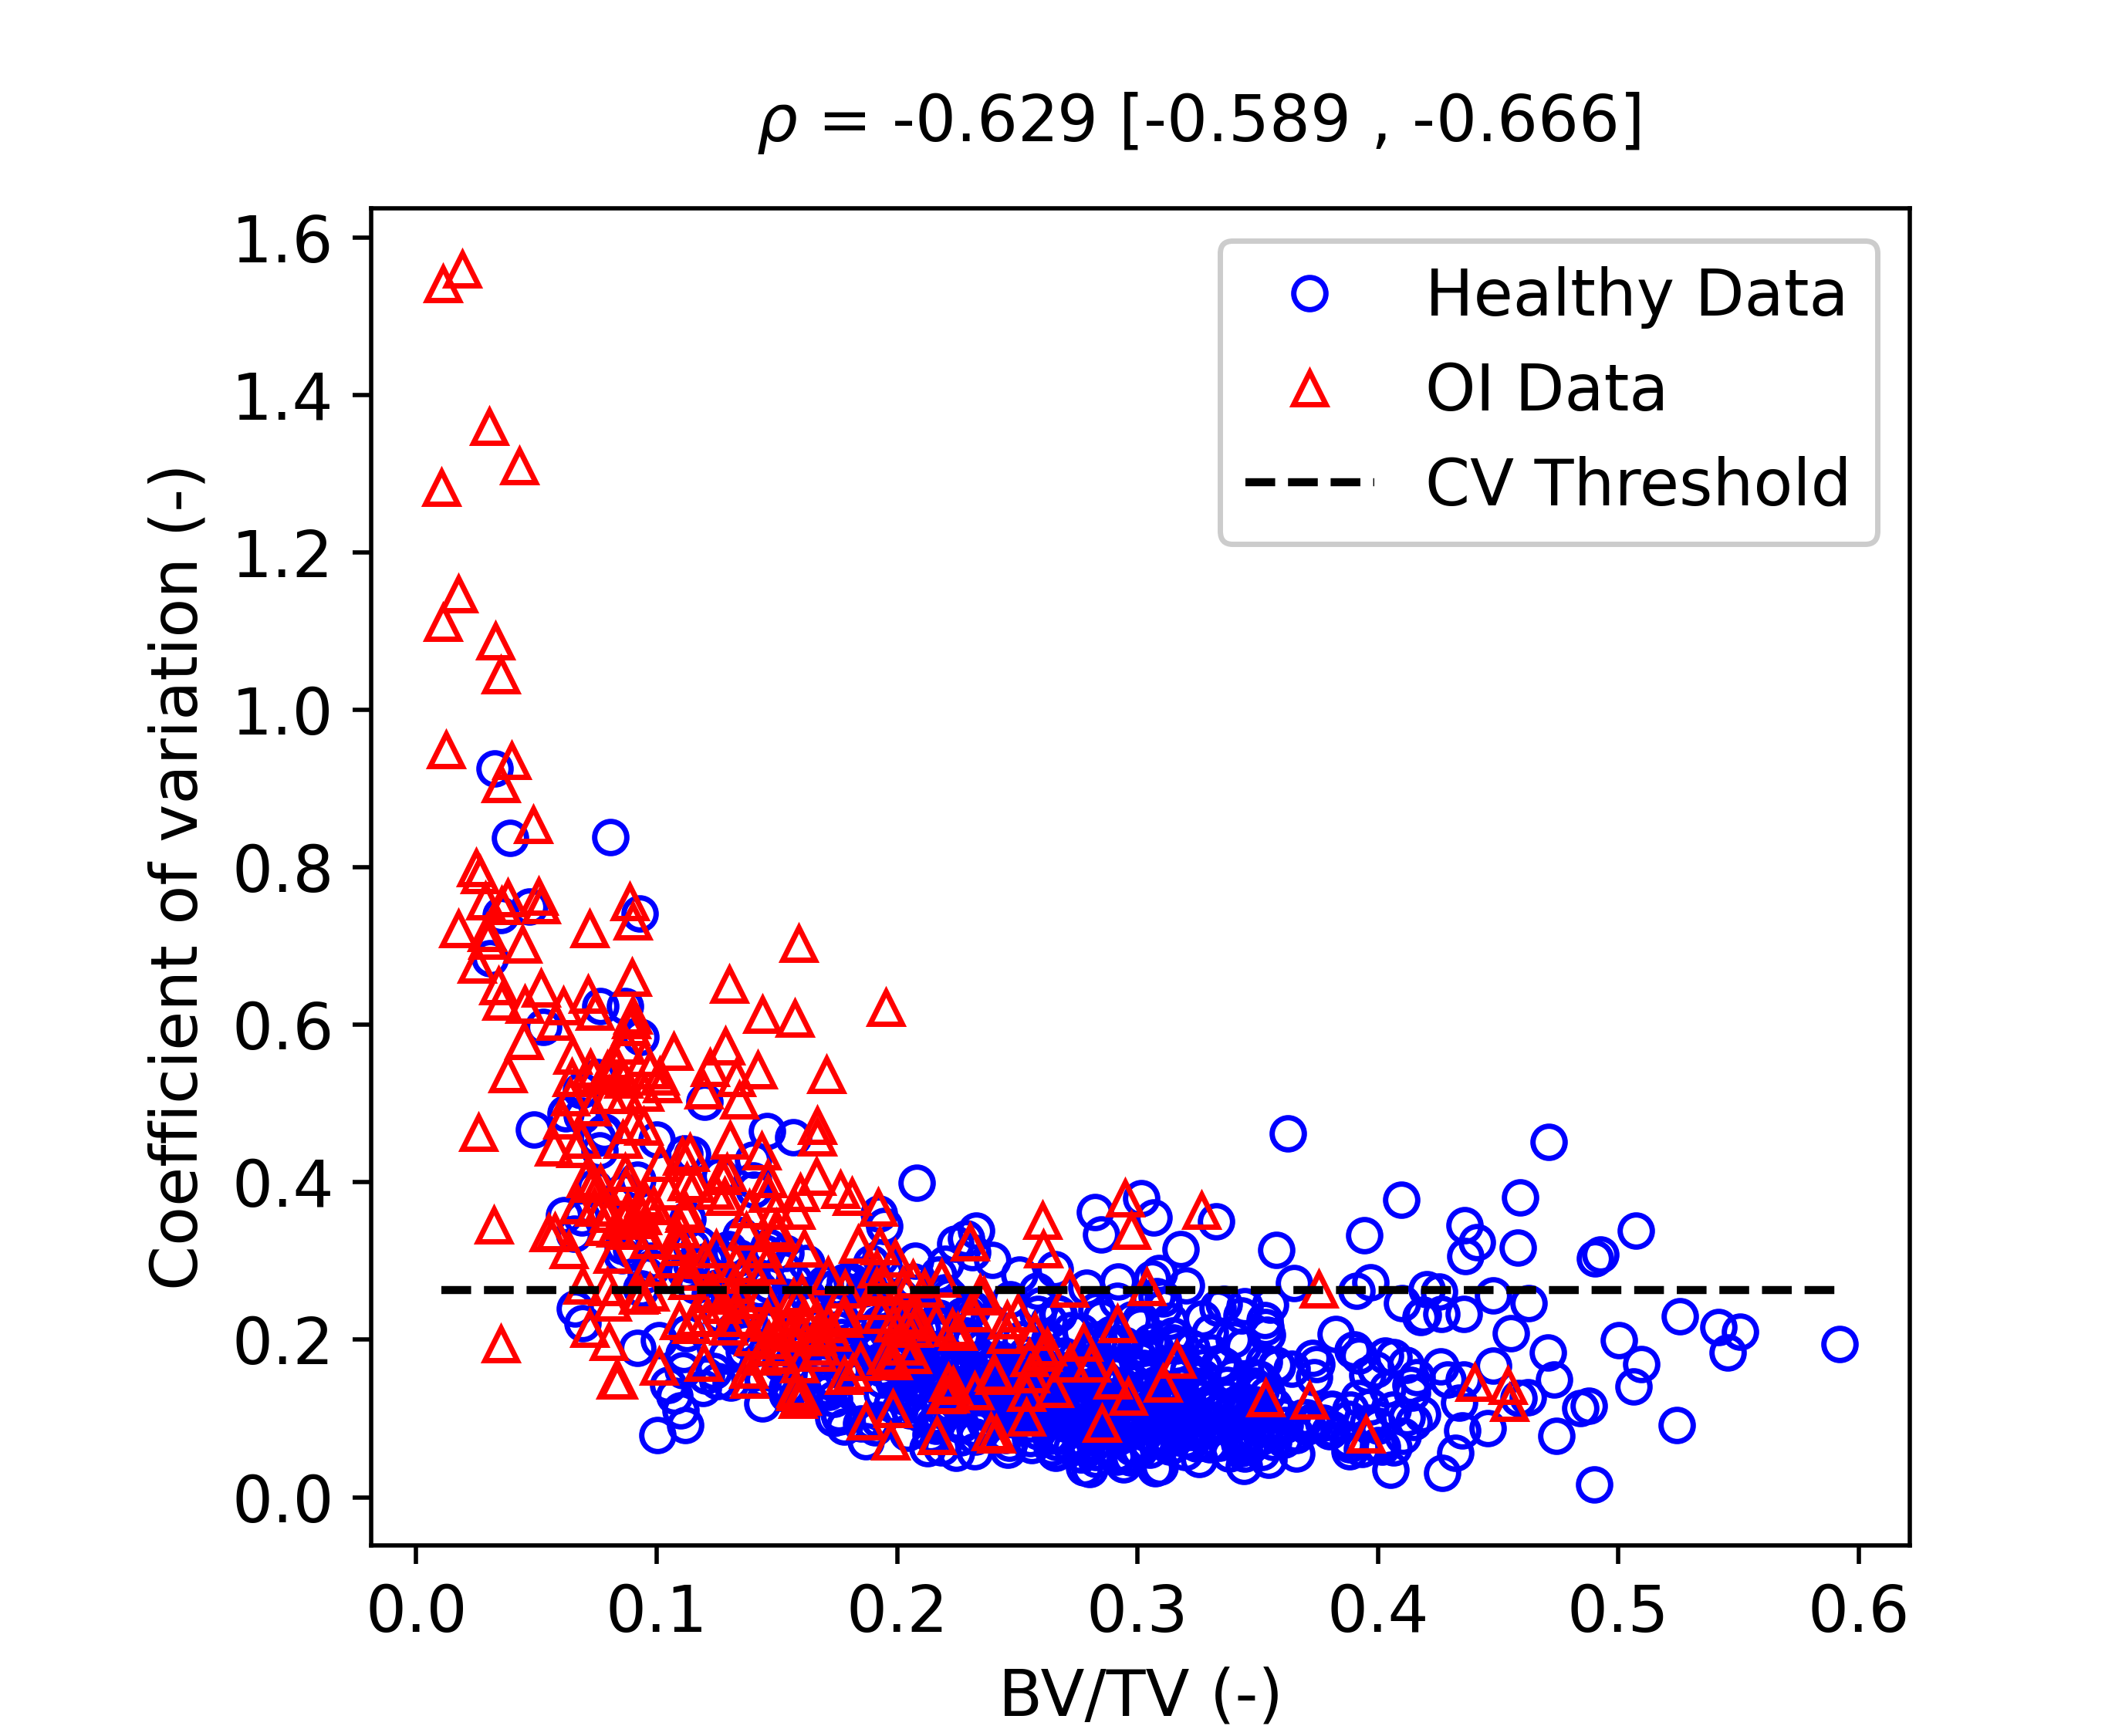
\includegraphics[height=0.425\linewidth]{../Trabecular/03_CV_BVTV}
	\end{frame}

	\begin{frame}
		\frametitle{Constitutive Models}
		\framesubtitle{Cortical ...}
		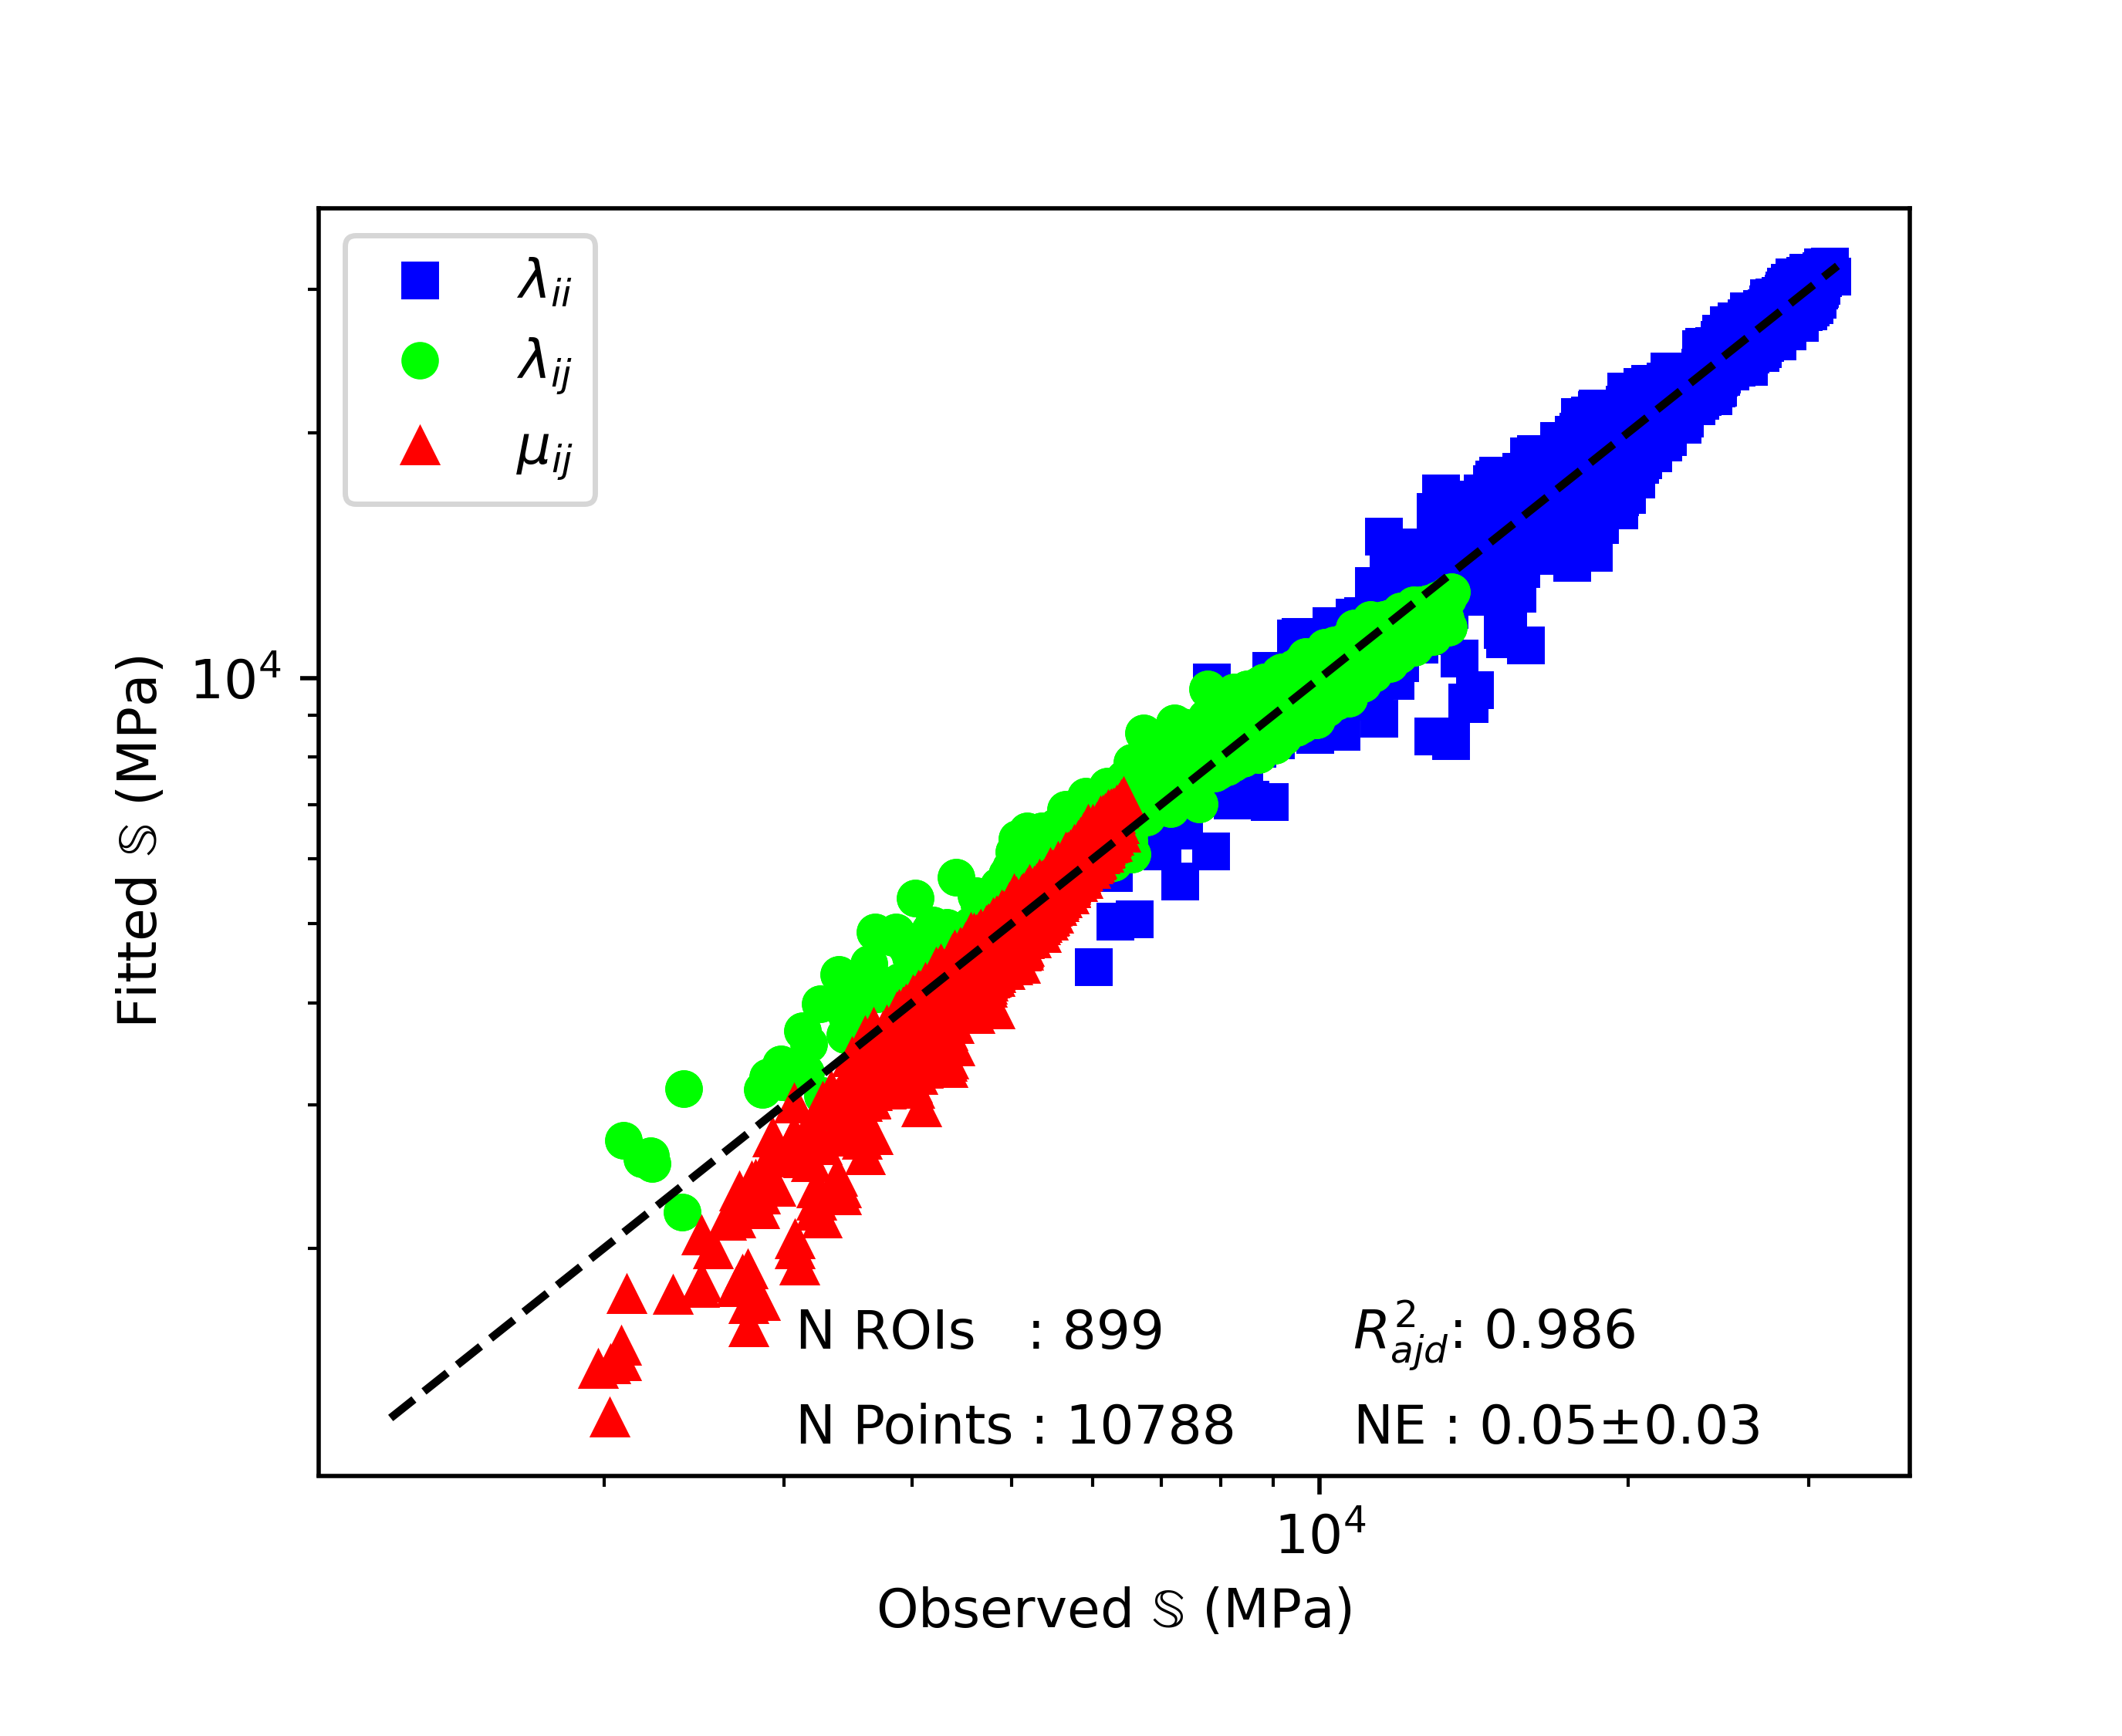
\includegraphics[width=0.32\linewidth, trim=20 0 20 0]{../Results/StandardOrthoModel}
		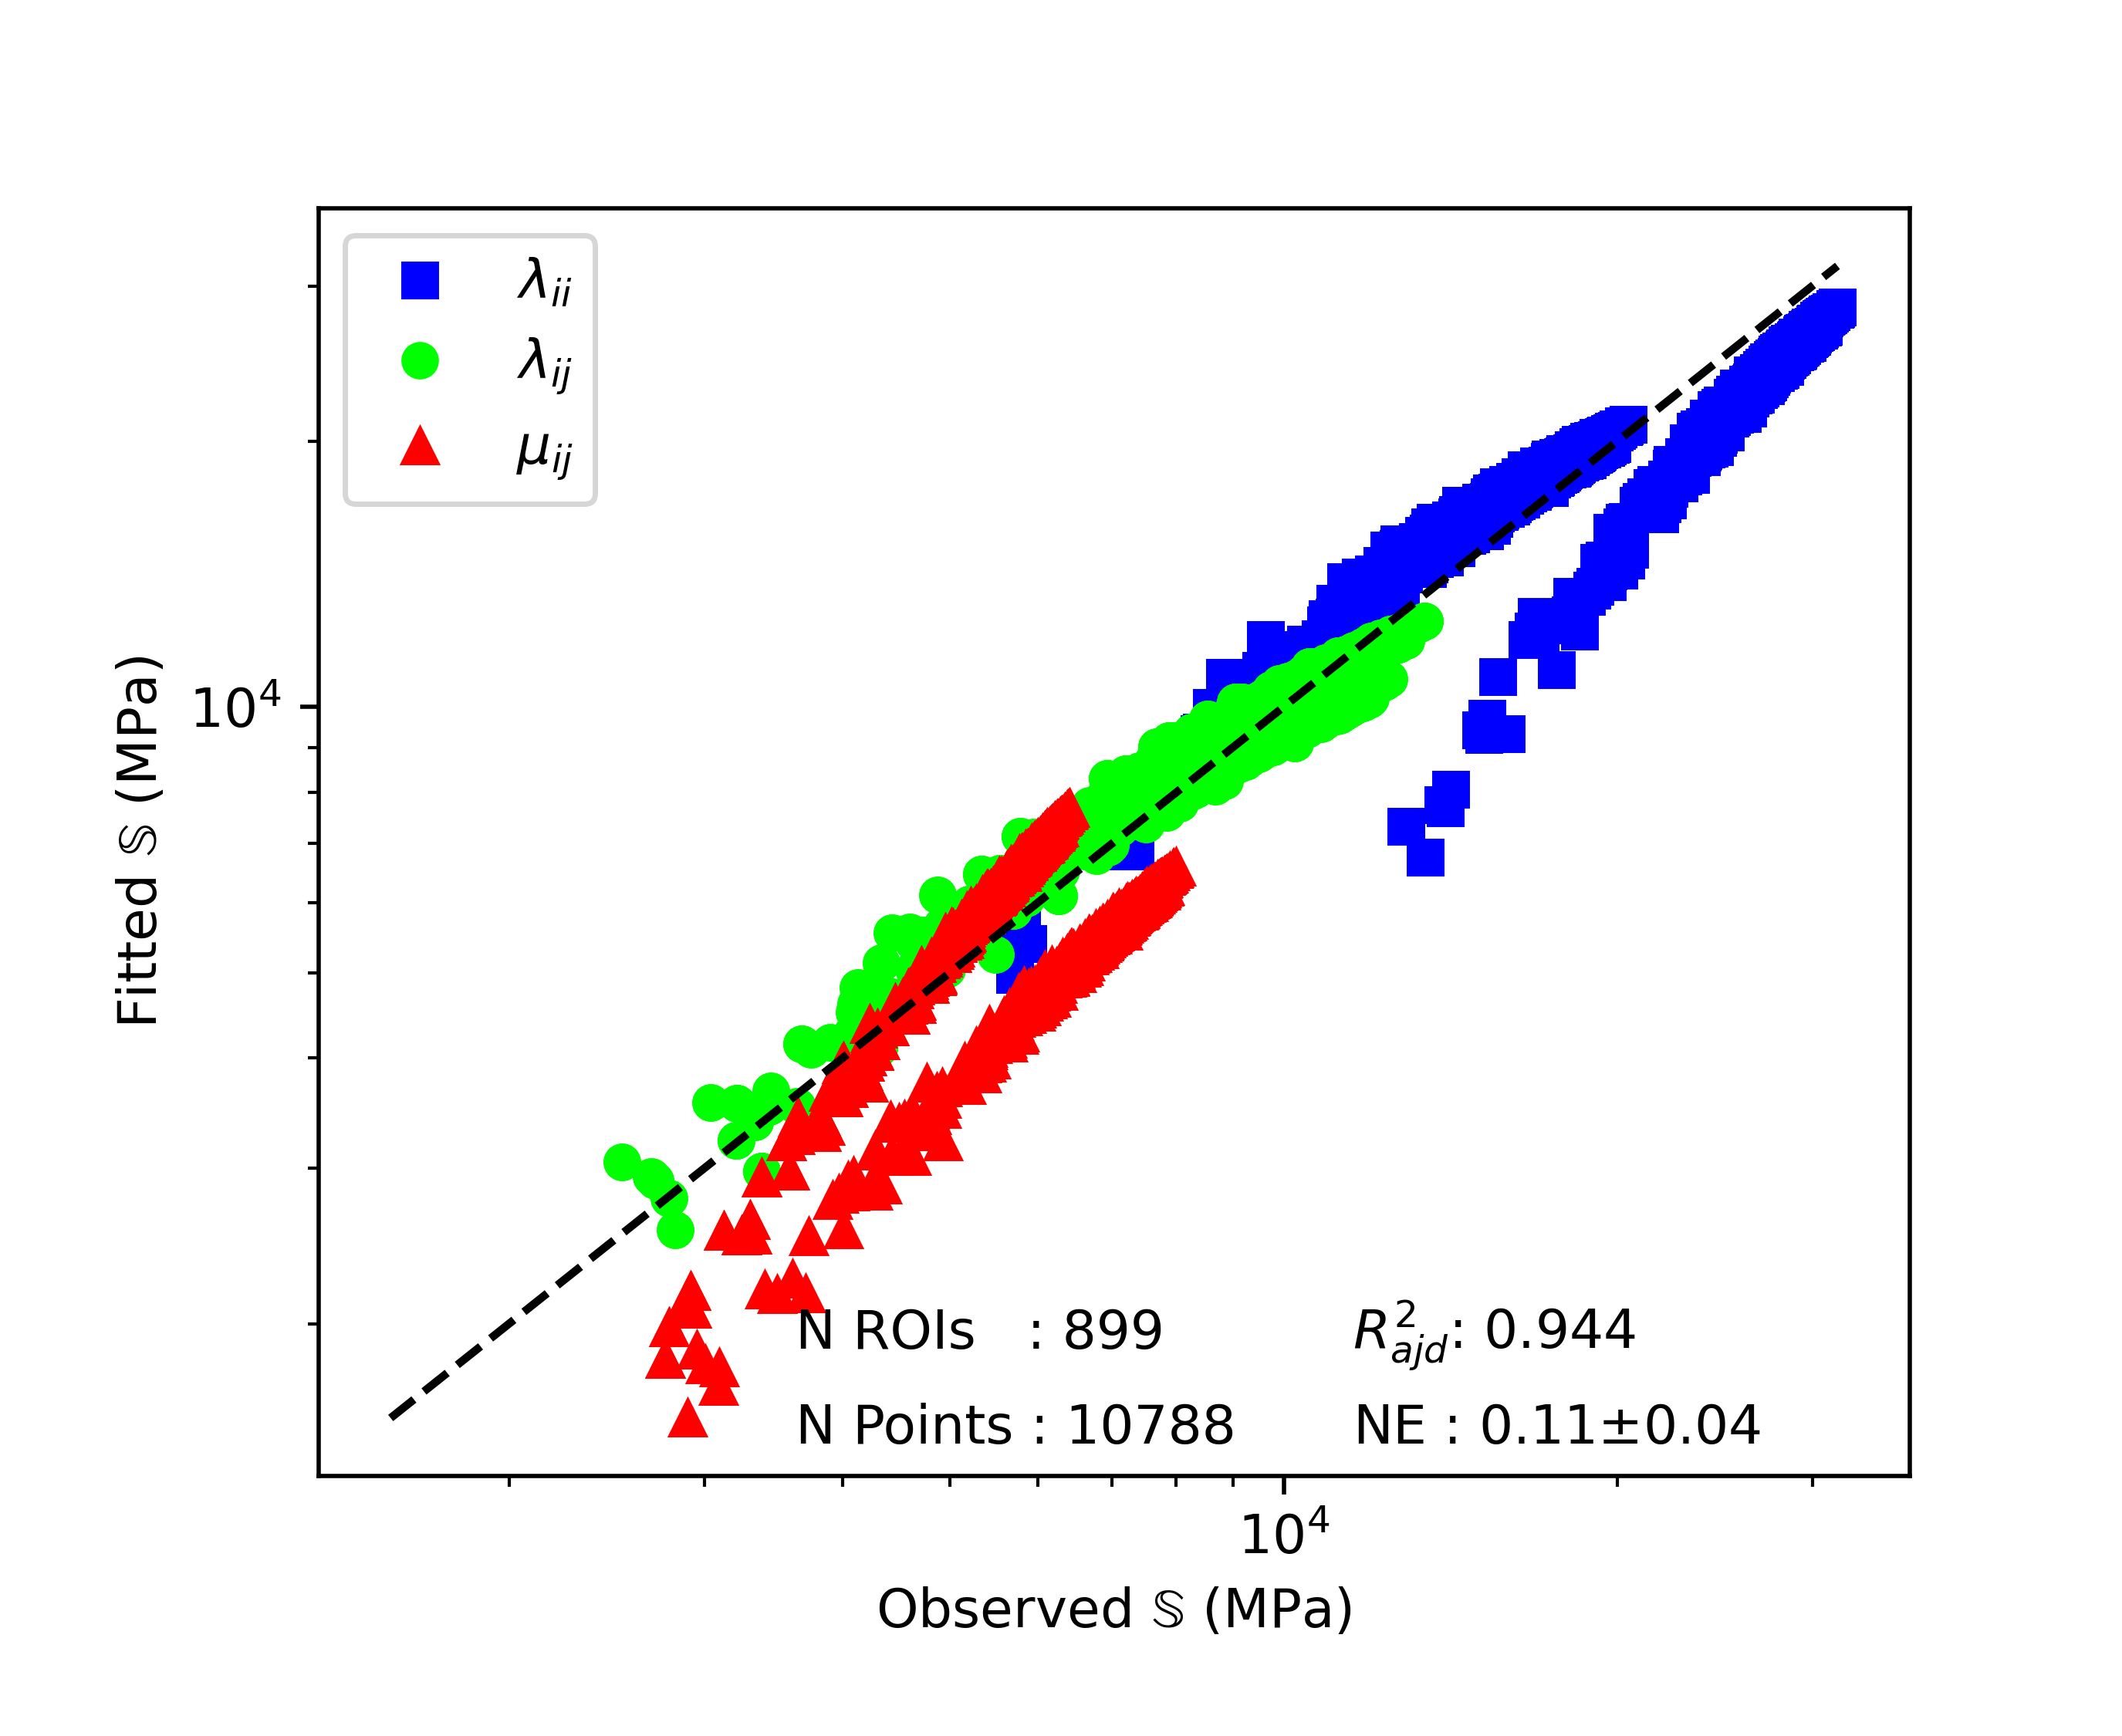
\includegraphics[width=0.32\linewidth, trim=20 0 20 0]{../Results/StandardTransModel}
		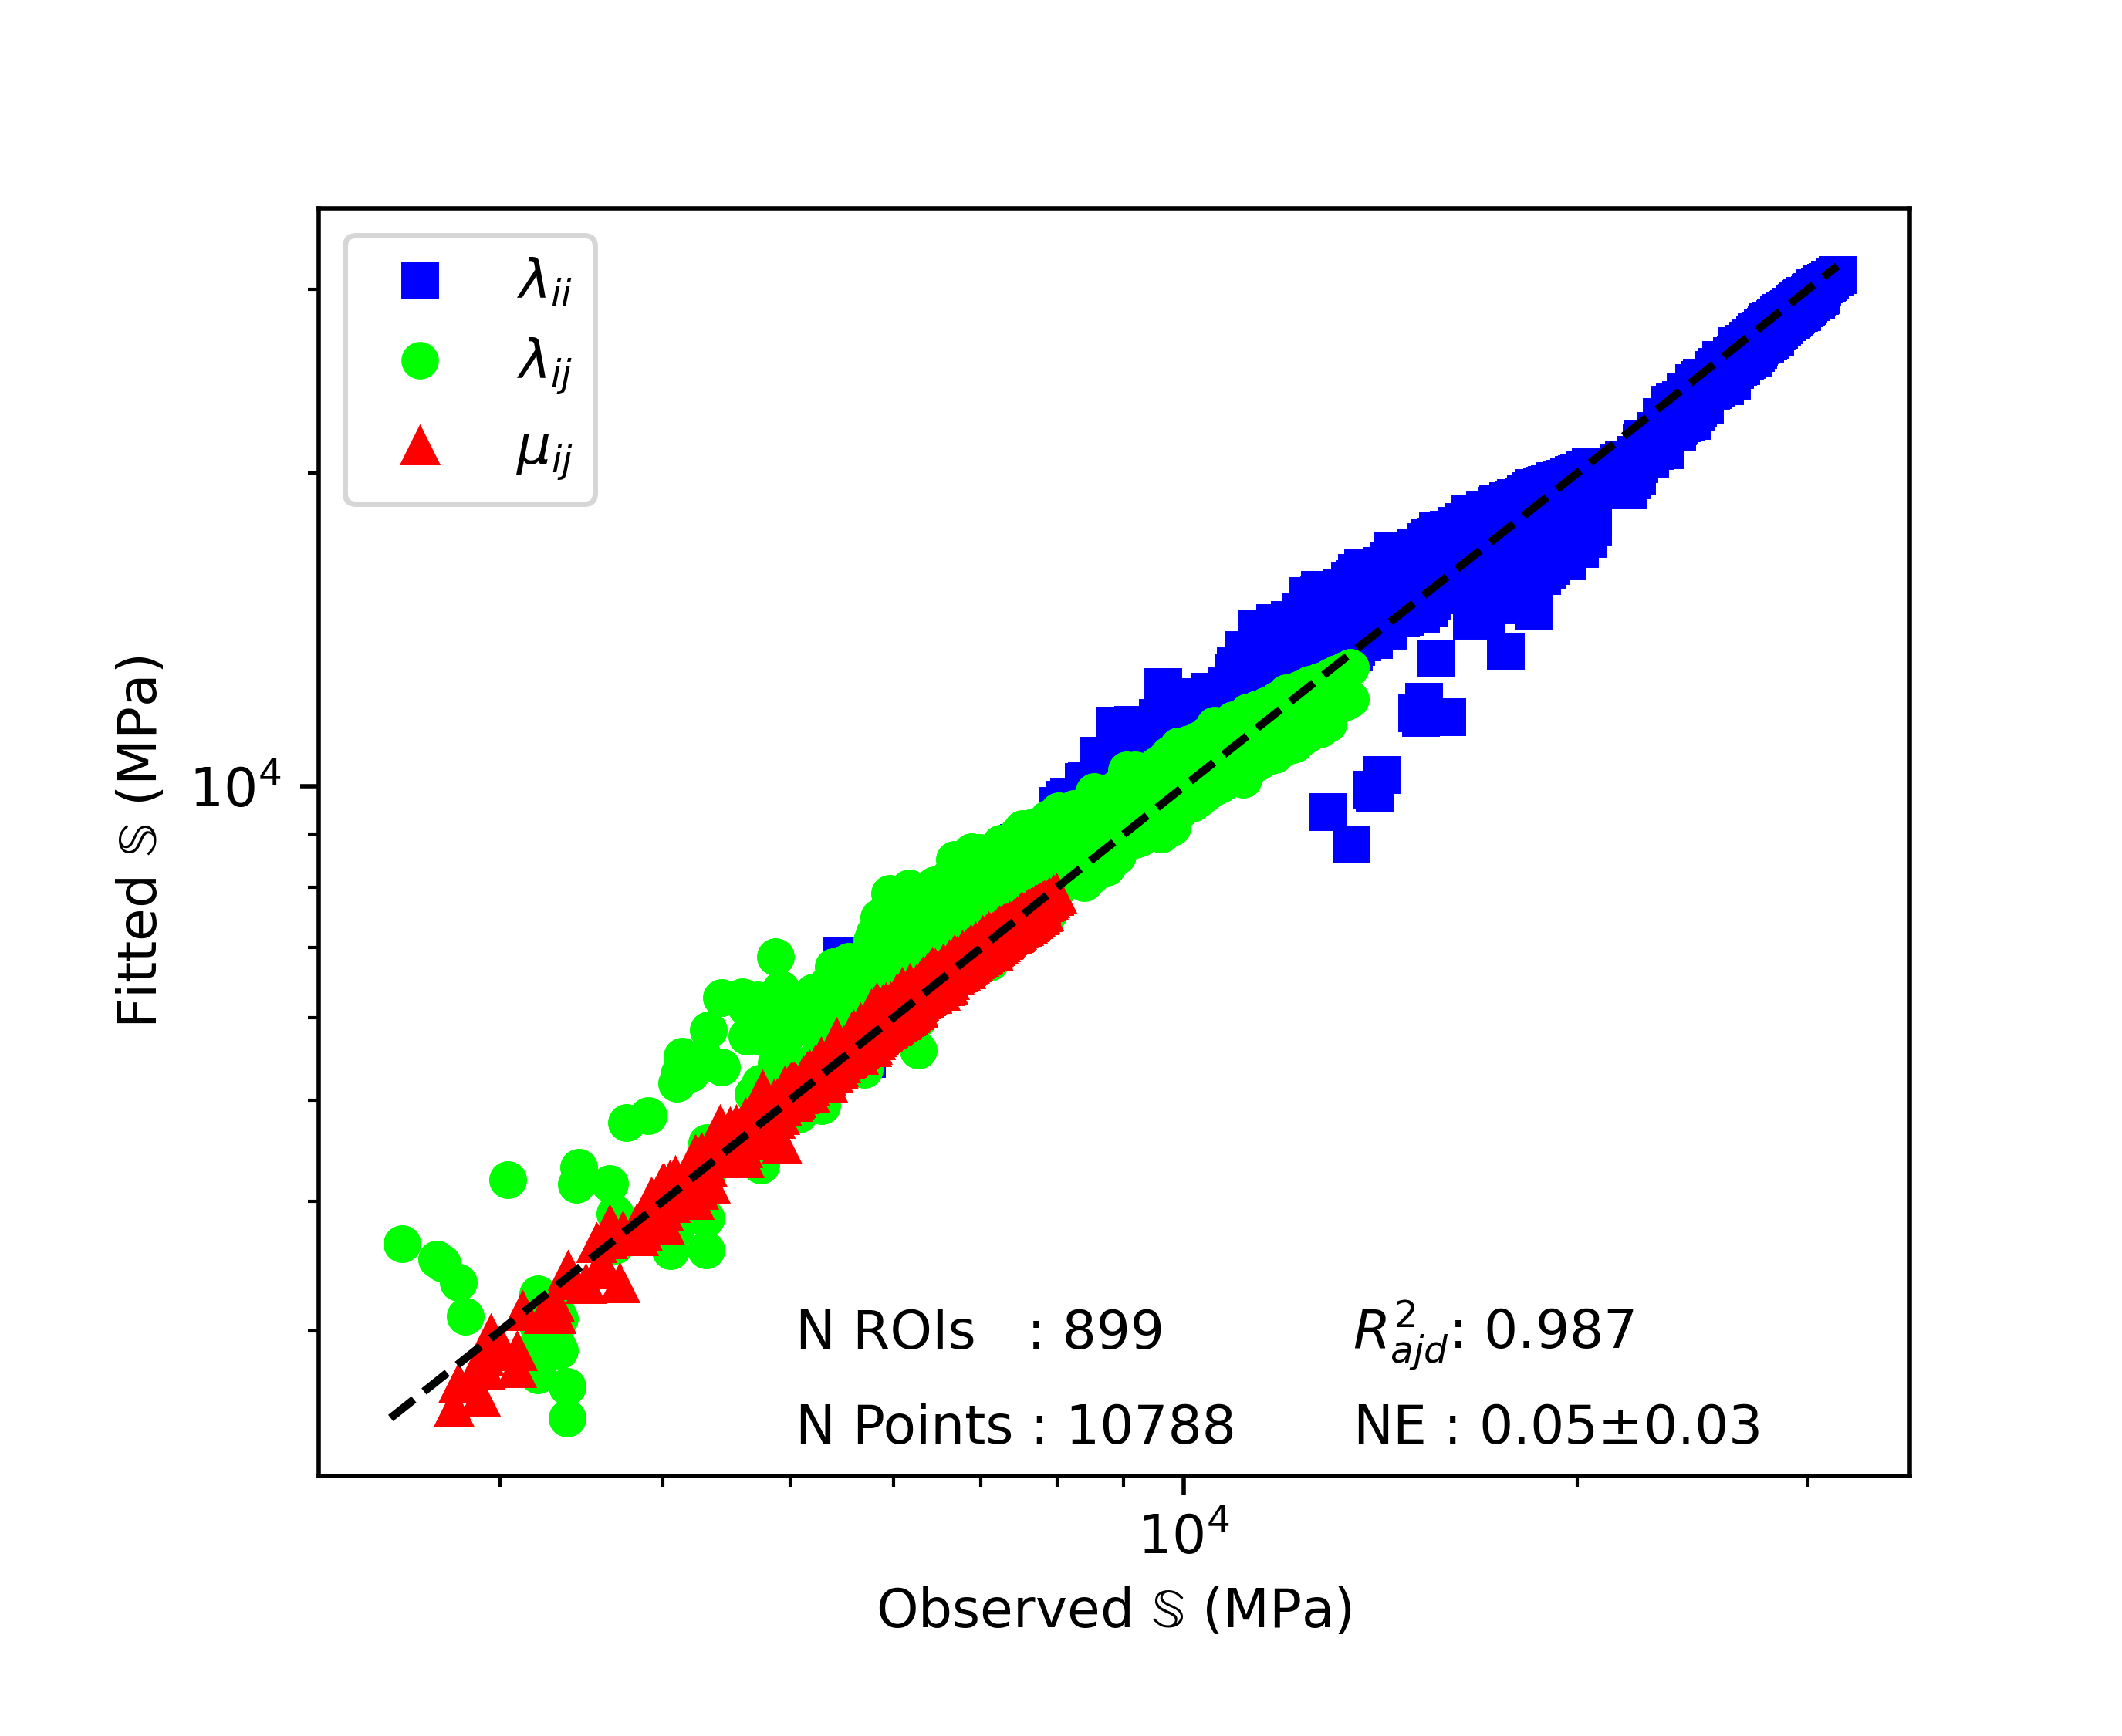
\includegraphics[width=0.32\linewidth, trim=20 0 20 0]{../Results/SpectralModel}
	\end{frame}

	\begin{frame}
		\frametitle{Constitutive Models}
		\framesubtitle{... to Trabecular}
		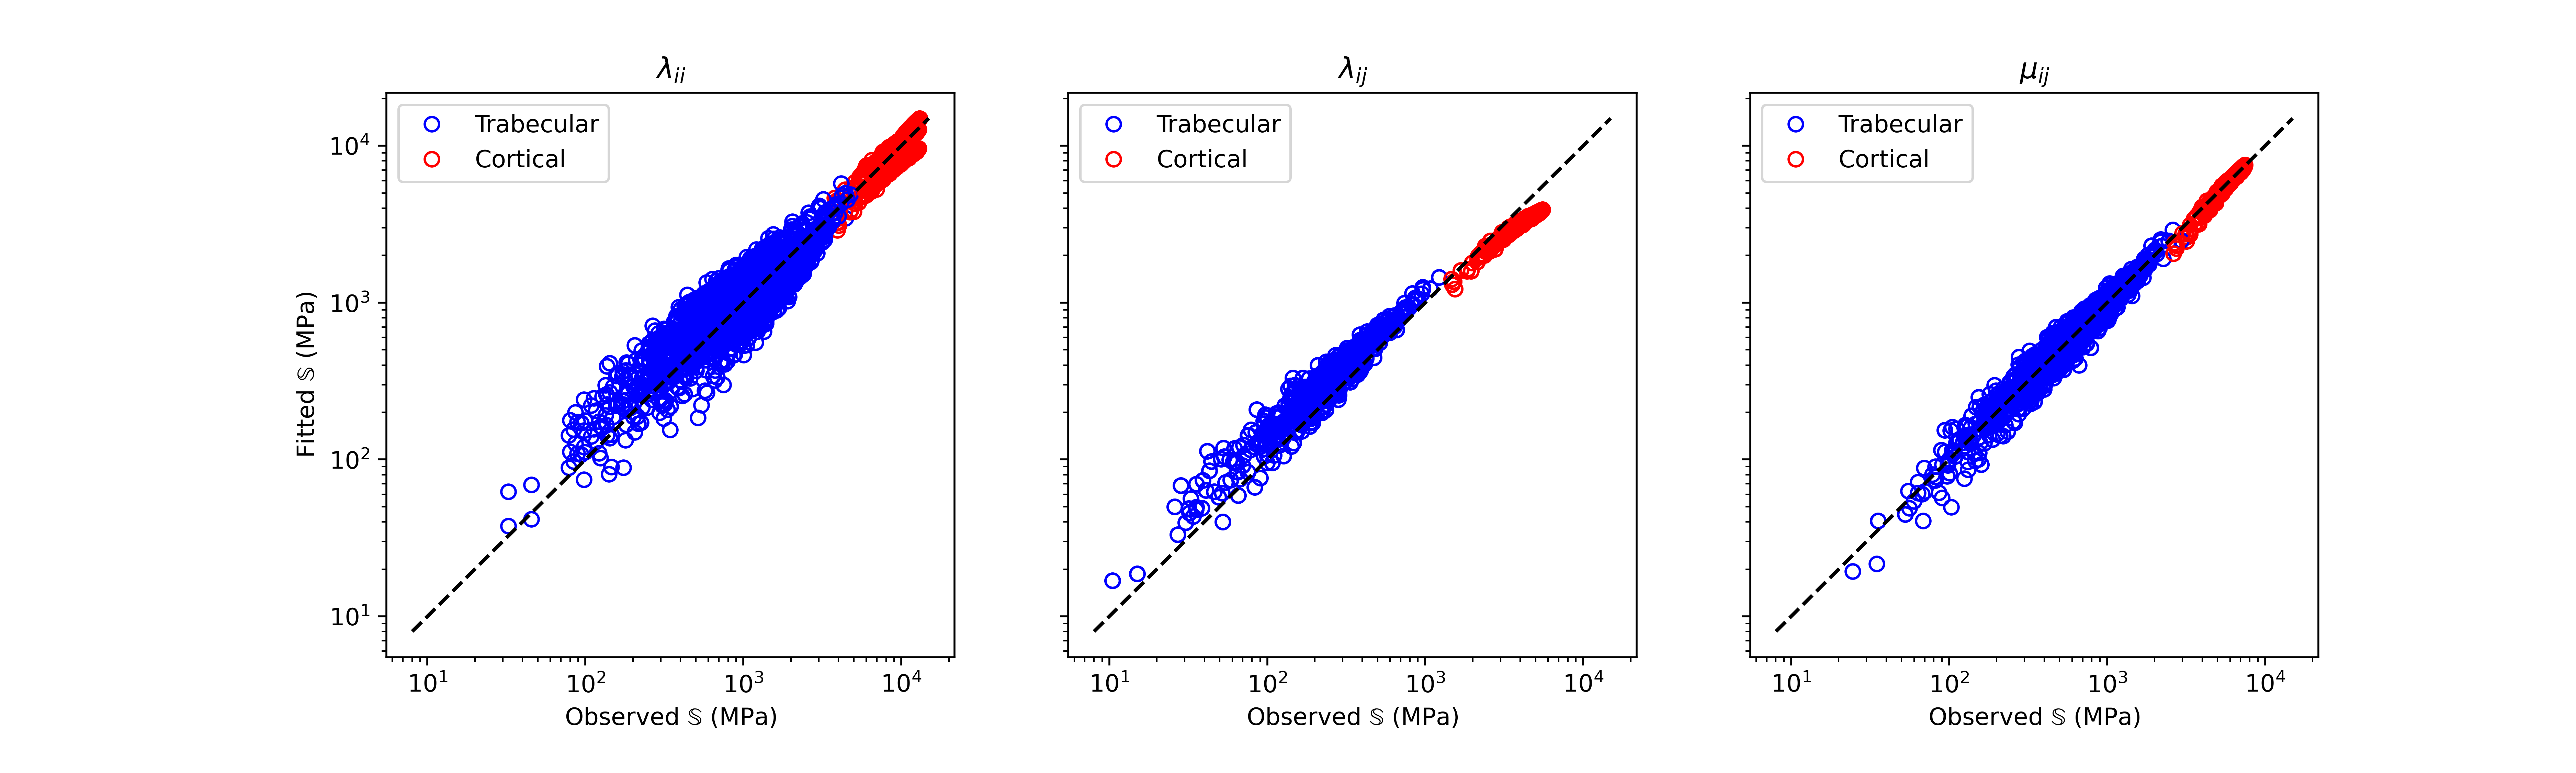
\includegraphics[width=1.1\linewidth, trim=100 0 0 0]{../Trabecular/SpectralModel}
	\end{frame}

	\begin{frame}
		\frametitle{Cortical and Trabecular Bone}
		\framesubtitle{Eigenvalues}
		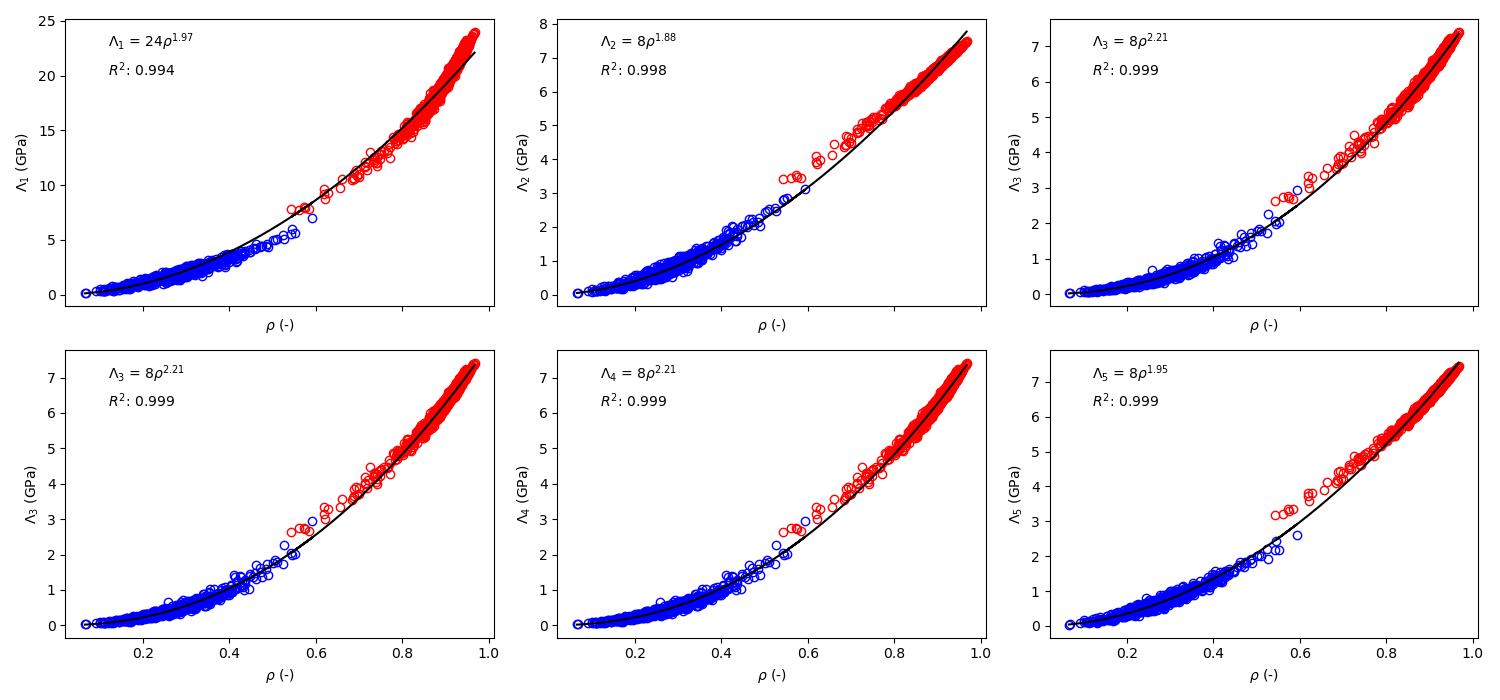
\includegraphics[width=\linewidth]{../Trabecular/LambdaVSRho}
	\end{frame}

	%----------------------------------------------------------------
	%----------------------------------------------------------------
	%----------------------------------------------------------------

	\section{References}

	\begin{frame}
		\frametitle{References}
		\footnotesize{
				\begin{thebibliography}{99}
						\setbeamertemplate{bibliography item}[triangle]
						
						\bibitem[1]{p1} Franzoso, G. and Zysset, P. (2009)
						\newblock Elastic anisotropy of human cortical bone secondary osteons measured by nanoindentation
						\newblock \textit{J Biomech Eng.}, 131(2)
						\newblock https://api.semanticscholar.org/CorpusID:25765365

						\bibitem[2]{p2}Enrico, D., Schmidt, R. and Zysset P. (2012)
						\newblock Microindentation can discriminate between damaged and intact human bone tissue
						\newblock \textit{Bone}, 50(4)
						\newblock https://api.semanticscholar.org/CorpusID:23349859
						
					\end{thebibliography}
			}
	\end{frame}
	
\end{document}